\section{Results}

\subsection{Large-scale self-supervised pretraining of \method{}}

Learning a reusable representation of the methylome requires a training signal that does not
depend on phenotype labels, because such labels are available for only a small and
inconsistently annotated fraction of public methylation profiles. We therefore pretrained
\method{} on 169,120 human DNA methylation profiles represented in a shared vocabulary of
49,156 CpG sites, without using chronological age, tissue, sex, dataset, or disease
annotations at any point in the objective (Fig.~\ref{fig:study-design}a). The corpus was
partitioned 80/10/10 by a fixed
permutation into 135,296 training, 16,912 validation, and 16,912 held-out profiles; the
held-out partition was never seen during pretraining and supports the reconstruction analyses
below.

Each profile generates two independently sampled views, each containing 50\% of its measured
CpGs. A shared encoder compresses each view into a 256-dimensional CLS representation, from
which a decoder predicts measured CpGs withheld from that view; a symmetric cross-view
contrastive term aligns the two CLS representations of one profile while separating
representations of different profiles (Fig.~\ref{fig:study-design}b--d). Because the two views are
drawn independently rather than as a partition, their expected overlap is half of the sites in
either view---equivalently, one quarter of all measured CpGs---a property we return to below.
The encoder architecture and token construction
are given in Methods and illustrated in Supplementary Fig.~S1.

Downstream evaluation used the AltuMAge-derived collection of 10,988 profiles measured at
21,368 CpGs. Two distinct populations were derived from it, and the distinction governs how
every subsequent result should be read. Frozen-representation diagnostics use the original
train/validation/test partition (7,416/1,308/2,264 profiles). The supervised age benchmark
applies a prespecified age filter and methylation-fingerprint deduplication, removing 328 age
outliers and 71 duplicates to leave 10,589 profiles, from which five stratified
training/validation folds (7,177/1,263) and one fixed test set of 2,149 unique samples were
constructed. Every fine-tuning and paired-comparison metric reported below uses that same
2,149-sample test set, for both model families and all five folds. Figure~\ref{fig:study-design}e
summarizes the two downstream evaluation modes considered here: supervised age fine-tuning and
frozen representation analysis.

% DRAFT FIGURE FOR MANUAL REVIEW. Before submission, replace this raster draft with a
% vector-native version and correct the four known visual issues: duplicated View A label;
% CpG embedding -> CpG identity embedding; remove the RoPE-to-V arrow; and move InfoNCE away
% from the downstream flow so that panel e originates from the pretrained encoder/global CLS.
\begin{figure}[!htbp]
 \centering
 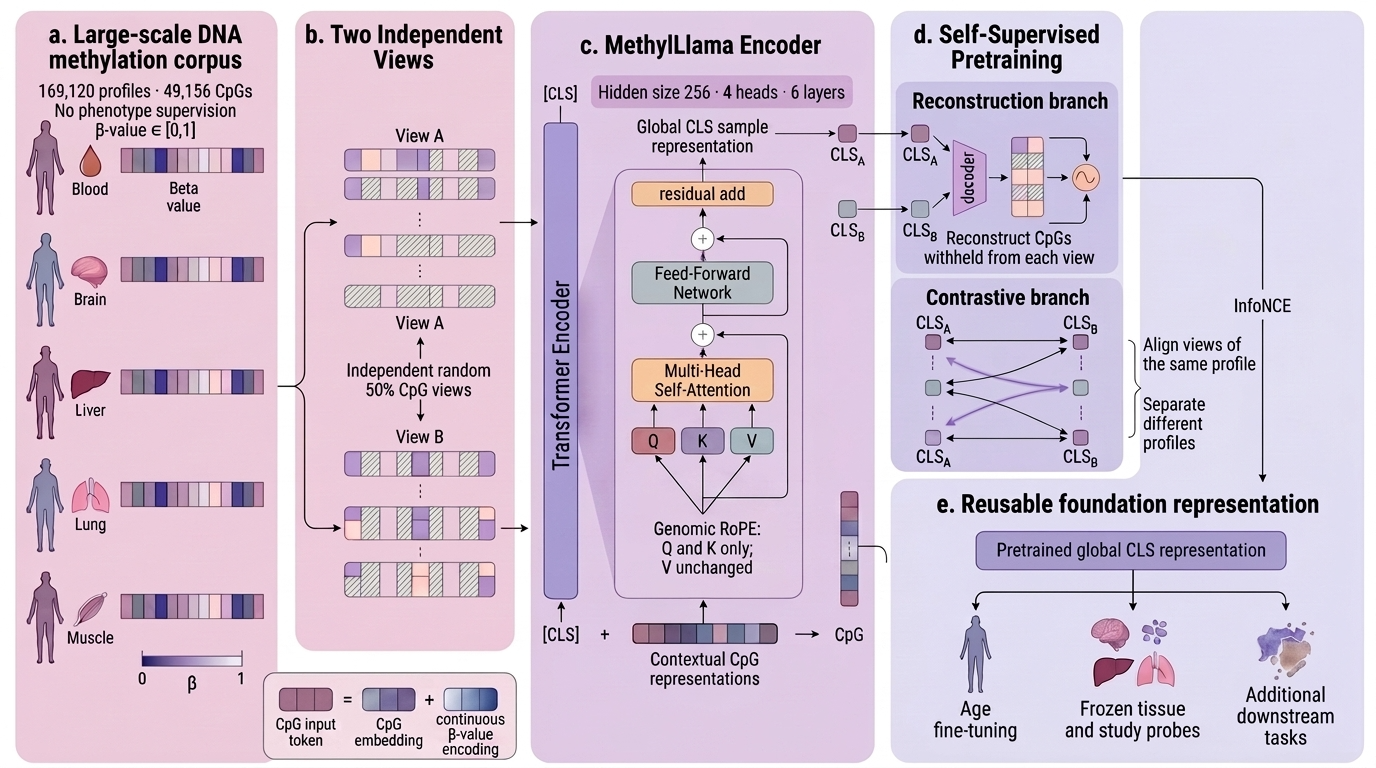
\includegraphics[width=\linewidth]{fig1_methylllama_overview_draft.png}
 \caption{\textbf{Overview of \method{} pretraining and downstream reuse.}
 \textbf{a}, The self-supervised pretraining corpus comprises 169,120 human DNA methylation
 profiles represented at 49,156 selected CpG sites; phenotype annotations do not enter the
 objective. \textbf{b}, Each profile is sampled into two independent random views, each retaining
 50\% of its measured CpGs. Coloured cells denote CpGs present in a view and hatched cells denote
 CpGs omitted from that view. \textbf{c}, A shared six-layer Transformer encoder combines CpG
 identity with continuous methylation-value encoding and summarizes each view in a global CLS
 representation. Genomic-rank rotary position encoding is applied to the query and key
 projections within self-attention, while the value projection is unchanged. \textbf{d}, WCED
 couples reconstruction and cross-view contrast: a shared decoder uses each CLS representation
 to predict measured CpGs withheld from the corresponding input, while a symmetric InfoNCE
 objective aligns the two views of one profile against representations of other profiles.
 \textbf{e}, The pretrained global representation is reused for supervised chronological-age
 fine-tuning and frozen tissue and study probes, with further downstream tasks left for future
 evaluation. The loss is
 $\mathcal{L}=\mathcal{L}_{\mathrm{recon}}+0.05\,\mathcal{L}_{\mathrm{InfoNCE}}$; additional
 architectural detail is provided in Supplementary Fig.~S1.}
 \label{fig:study-design}
\end{figure}

\subsection{WCED learns sample-specific representations from partial methylation profiles}

If the CLS bottleneck is to serve as a reusable sample representation, it must satisfy two
requirements that pull in opposite directions: it must be stable when a different subset of the
methylome is observed, and it must remain specific enough to distinguish one profile from
another. We tested both directly.

Across five independent random draws of two half-profile views for each of 2,000 profiles,
matched views had a mean cosine similarity of $0.984\pm0.0004$ against $0.499\pm0.0002$ for
unmatched profiles, and the correct partner view was retrieved as the nearest neighbour for
73.8\% of queries (range 73.1--74.5\% across draws; chance 0.05\%), rising to 96.1\% within the
ten nearest candidates (Fig.~\ref{fig:partial-view}a,b). The representation is therefore stable
under random 50\% CpG subsampling while remaining specific to the individual profile.

Part of that stability is supplied by shared input rather than by the representation itself.
Repeating the evaluation with strictly disjoint views---a random partition in which the two
halves share no site---left mean matched similarity almost unchanged ($0.971\pm0.0005$ versus
$0.984$) but reduced top-1 retrieval to 25.3\% (range 24.6--26.0\%). The dissociation is
informative: mean similarity is insensitive to the change, whereas identifying the correct
partner among 1,999 competitors depends on narrow margins against the most similar profiles,
which the small loss of positive similarity is sufficient to erase. Cross-subset identity
information is clearly retained---disjoint-view retrieval remains roughly 500-fold above chance
and reaches 75.1\% within ten candidates---but it is weaker than the overlapping-view figure
alone implies. The encoder was trained with overlapping views, so the disjoint condition is out
of distribution for it and these values are a conservative bound rather than an estimate of
what the architecture achieves when trained for that regime (Supplementary Fig.~S2).

A related question is whether a profile assayed at fewer sites embeds where its complete
profile does. The embedding of a random 50\% CpG subset had mean cosine similarity 0.991 to the
embedding of its own complete profile (shuffled-pairing control, 0.496), and a ridge age probe
fitted on complete-profile embeddings and applied without adaptation to subset embeddings of
held-out profiles retained $R^2=0.835$ against $R^2=0.863$ on complete profiles (paired
difference 0.028, 95\% CI 0.014--0.044; Supplementary Fig.~S3). These are random CpG subsets
rather than the probe set of a particular array generation, so the result indicates robustness
to which sites are observed and does not by itself establish transfer across measurement
platforms.

We then asked whether the CLS bottleneck carries enough information to recover methylation
values the encoder never saw. Reconstruction was evaluated on 5,000 profiles from the held-out
partition of the pretraining corpus, encoding each from a 50\% subset of its measured CpGs and
scoring predictions only at measured CpGs absent from that input ($1.12\times10^{8}$ evaluated
positions). Predicted and observed beta values were closely correlated (Pearson $r=0.972$,
computed on a random sample of approximately $5.0\times10^{5}$ withheld positions), and the
per-profile standardized reconstruction loss, computed over all withheld positions, was 0.0525
(Fig.~\ref{fig:partial-view}c).

To test whether the decoder reads the sample representation rather than exploiting
population-level regularities, we compared three controls on the same profiles under identical
withheld masks. Mean squared error at withheld CpGs was 0.0056 for the model, against 0.0306
for a per-CpG mean predictor, 0.0505 for a decoder given standard normal vectors, and 0.0552
for a decoder given CLS embeddings shuffled across the batch. The paired per-profile difference
against every control excluded zero (Fig.~\ref{fig:partial-view}d), and the model reduced error
5.4-fold relative to the per-CpG mean even though that baseline was computed on the evaluation
cohort itself and is therefore advantaged. Shuffled CLS embeddings produced slightly worse
reconstruction than random vectors, indicating that a real but mismatched sample representation
is more misleading than no sample information at all. Together with cross-view retrieval, this
establishes that the CLS bottleneck carries sample-specific information sufficient both to
identify a profile and to predict methylation values never supplied to the encoder.

\begin{figure}[!htbp]
 \centering
 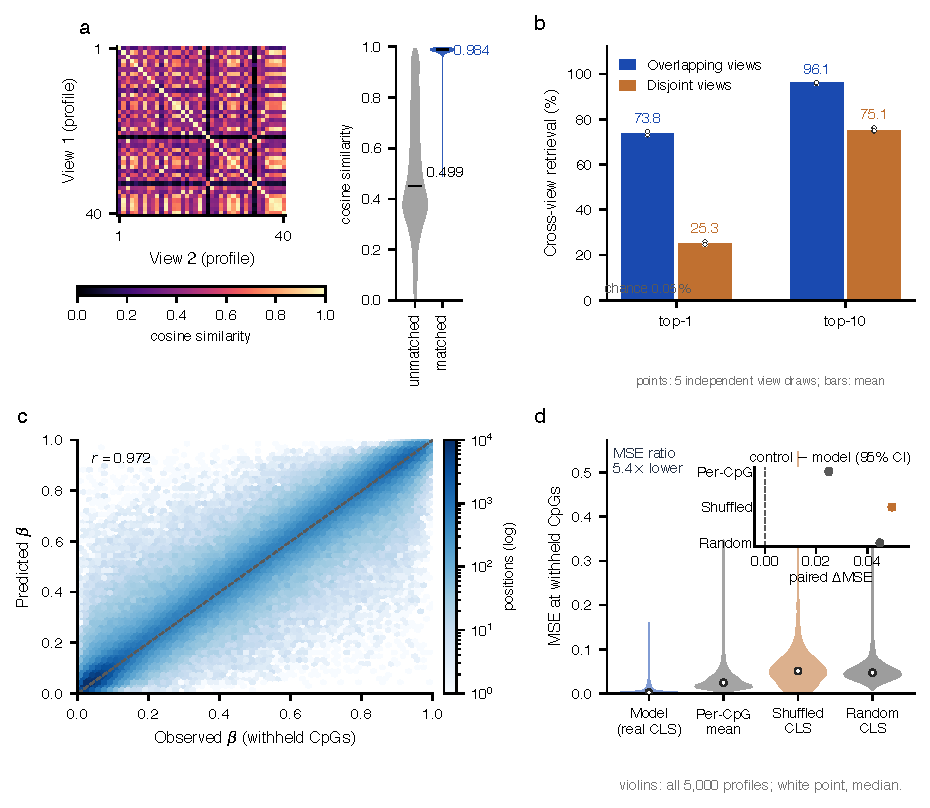
\includegraphics[width=\linewidth]{fig2_wced_consistency_reconstruction.pdf}
 \caption{\textbf{WCED learns view-stable, sample-specific representations that reconstruct
 withheld CpGs.} \textbf{a}, Cosine similarity between CLS embeddings of two independently
 sampled 50\%-CpG views. Heatmap: 40 profiles drawn at random under a fixed seed; the bright
 diagonal marks matched views of the same profile, and the two dark rows are
 individual profiles with genuinely low similarity to the rest of the draw
 rather than missing data. Violins: all 2,000 profiles of one draw,
 means annotated. \textbf{b}, Cross-view retrieval accuracy against the number of candidates
 considered, for overlapping and disjoint view constructions, with chance shown. Points give
 the mean across five independent view draws and vertical lines their range; top-1 and top-10
 are annotated. \textbf{c}, Observed versus predicted $\beta$ at CpGs withheld from the encoder
 input, for 5,000 profiles of the held-out pretraining partition (hexagonal binning,
 logarithmic colour scale; dashed line, identity). The panel displays a random sample of
 approximately $5.0\times10^{5}$ of the $1.12\times10^{8}$ evaluated positions, and the
 reported $r=0.972$ was computed on that sample; reconstruction-error summaries in \textbf{d}
 were computed over all withheld positions. \textbf{d}, Per-profile mean squared error at
 withheld CpGs for the model and three controls evaluated on the same 5,000 profiles under
 identical withheld masks (violins, all profiles; white point, median). Inset: paired
 control-minus-model differences with 95\% bootstrap confidence intervals over 10,000 resamples
 of profiles; the statistical unit is the profile.}
 \label{fig:partial-view}
\end{figure}

\subsection{Self-supervised pretraining captures biologically informative variation}

Pretraining optimized reconstruction and cross-view agreement, neither of which references
biology. We therefore asked what biological information the frozen representation nonetheless
contains, using linear probes fitted on the original AltuMAge partition (8,724 profiles for
fitting, 2,264 for evaluation) with no update to the encoder.

A ridge regressor on frozen CLS embeddings predicted chronological age with $R^2=0.866$ and a
median absolute error of 5.17 years. Applying the same probe to mean-pooled contextual CpG
embeddings from the same model reduced performance to $R^2=0.795$ and MedAE 6.53 years
(Fig.~\ref{fig:representation-generalization}a). The CLS space also had a higher effective rank
than the mean-pooled space and lower mean cosine anisotropy (Supplementary Table~S2). The
explicit sample token therefore retains broader and more age-informative variation than uniform
pooling over CpG tokens, despite receiving no age supervision.

Biological information was not restricted to age: a linear classifier on frozen CLS embeddings
attained balanced accuracy 0.936 across 37 sufficiently represented tissue classes (2,197
evaluation profiles; chance 0.027). These probes establish that biologically associated
structure is linearly accessible in the pretrained representation under an in-distribution
sample split. They do not show that biology has been separated from study or platform effects,
because profiles from the same study can fall on both sides of this split---a question we
address below.

\subsection{\method{} improves age prediction under a matched benchmark}

We next asked whether \method{} supports accurate chronological-age prediction under a matched
benchmark. Five models were fine-tuned on different stratified
training/validation folds and every selected checkpoint was evaluated on the same fixed
2,149-sample test cohort (age range 0--103 years; mean 45.53 years). Across folds, mean MedAE
was $3.169\pm0.040$ years, mean MAE $4.493\pm0.059$ years, and mean $R^2$ $0.9316\pm0.0024$
(mean $\pm$ sample SD; per-fold values in Supplementary Table~S1). Because all five models were
evaluated on the same samples, this dispersion measures sensitivity to the supervised training
partition and is not a confidence interval for population performance
(Fig.~\ref{fig:age-benchmark}a). Averaging the five predictions per sample gave the primary
\method{} estimate: MedAE 3.112 years, MAE 4.333 years, $R^2=0.9365$. MethylGPT was evaluated
using the same fold assignments, held-out subjects, and fold-ensemble aggregation.

The comparison used identical held-out samples, age labels, and fold assignments for both model
families, and uncertainty was estimated by resampling the same test samples for both models.
Throughout the text, table and figure, differences are signed so that positive values favour
\method{}: error differences are comparator minus \method{}, and $R^2$ differences are
\method{} minus comparator. \method{} reduced MedAE by 0.589 years (95\% CI 0.338--0.815) and
MAE by 0.773 years (0.583--0.968) relative to MethylGPT, and increased $R^2$ by 0.0254
(0.0183--0.0329); all three intervals excluded zero
(Table~\ref{tab:age-benchmark}, Fig.~\ref{fig:age-benchmark}b,c,d).

We additionally evaluated a conventional linear reference using ElasticNetCV \citep{Zou2005},
with hyperparameters selected by internal cross-validation on the pooled training and validation
profiles and the common test set withheld until final evaluation. The resulting model used
1,036 non-zero coefficients among 21,368 CpGs and achieved MedAE 3.437 years, MAE 4.731 years,
and $R^2=0.9322$. The \method{} ensemble had better point estimates than both comparators on
this test set. Because ElasticNet was evaluated as a single fitted model whose sample-level
predictions were not retained, that comparison is descriptive and carries no paired confidence
interval.

The benchmark is matched at the sample and split levels, but the two pipelines differ in their
treatment of 1,760 CpGs outside the shared pretraining reference: \method{} retains their
measured values under a common unknown-CpG identity, whereas MethylGPT excludes them. The
result therefore establishes a predictive advantage for the implemented \method{} pipeline as a
whole, and does not isolate the contribution of the WCED objective; an ablation that varies the
pretraining objective while holding the pipeline fixed would be required for that attribution.

\begin{table}[!htbp]
\centering
\caption{\textbf{Age prediction on the common 2,149-sample held-out test set.}
The first three rows are test-set point estimates. \method{} and MethylGPT are five-fold
prediction ensembles; ElasticNetCV is a single model selected by internal cross-validation.
The MethylGPT comparison row reports paired improvement of \method{} with 95\% bootstrap confidence
intervals over 10,000 resamples of the test samples, signed so that positive values favour
\method{} for all three endpoints ($\Delta$ error $=$ comparator $-$ \method{};
$\Delta R^2 = $ \method{} $-$ comparator). ElasticNet sample-level predictions were not
retained, so its improvement row is descriptive and has no paired interval.}
\label{tab:age-benchmark}
\small
\begin{tabular}{@{}lccc@{}}
\toprule
Model or comparison & MedAE (years) & MAE (years) & $R^2$ \\
\midrule
\method{} (five-fold ensemble) & 3.112 & 4.333 & 0.9365 \\
ElasticNetCV (single model) & 3.437 & 4.731 & 0.9322 \\
MethylGPT (five-fold ensemble) & 3.701 & 5.105 & 0.9110 \\
\midrule
\shortstack[l]{Improvement over MethylGPT\\(paired)} & $0.589\ [0.338,\,0.815]$ &
$0.773\ [0.583,\,0.968]$ & $0.0254\ [0.0183,\,0.0329]$ \\
\shortstack[l]{Improvement over ElasticNetCV\\(descriptive)} & $0.325$ & $0.398$ & $0.0043$ \\
\bottomrule
\end{tabular}
\end{table}

\begin{figure}[!htbp]
 \centering
 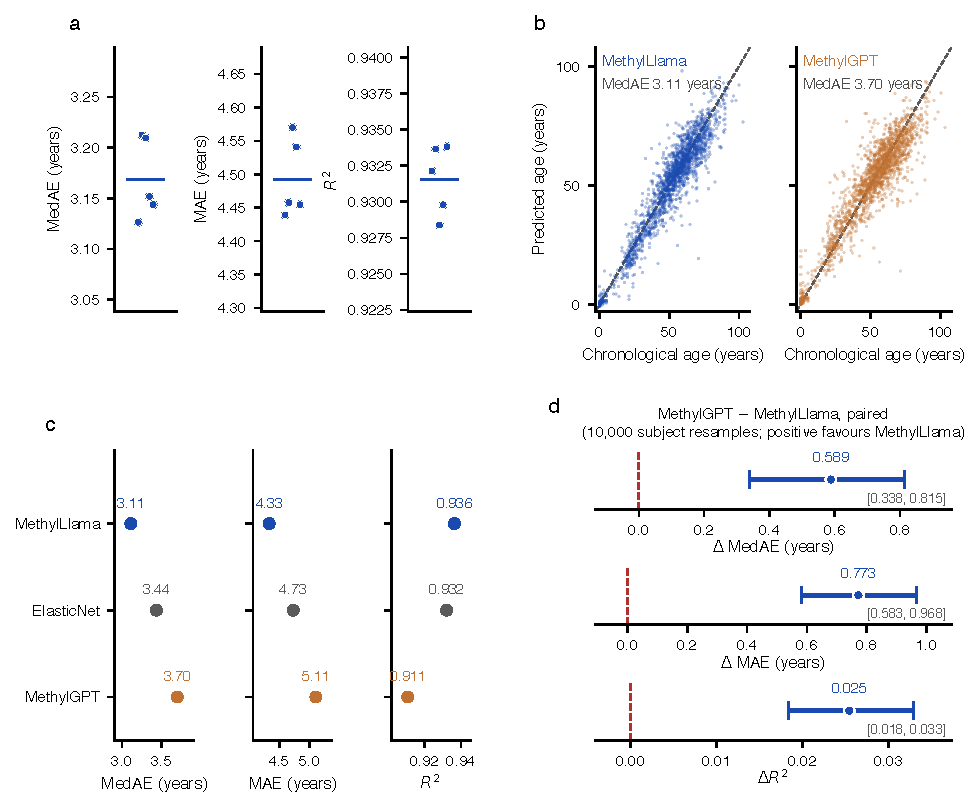
\includegraphics[width=\linewidth]{fig3_age_benchmark_paired_comparison.pdf}
 \caption{\textbf{Age prediction is stable across supervised partitions and improves on matched
 neural and linear references.} \textbf{a}, Stability across five supervised training
 partitions. Each point is one fine-tuned model evaluated on the same fixed 2,149-sample test
 cohort; horizontal lines are the means across partitions. The spread reflects sensitivity to
 the training partition, not population uncertainty, because the test samples are shared.
 \textbf{b}, Ensemble-predicted versus chronological age for \method{} and MethylGPT on the
 same 2,149 samples, on identical axes and scales; each point is one sample and dashed lines
 indicate identity. \textbf{c}, Ensemble point estimates for \method{} and MethylGPT with the
 single-model ElasticNetCV reference. \textbf{d}, Paired differences against \method{} with
 95\% bootstrap confidence intervals over 10,000 resamples of the test samples, signed so that
 positive values favour \method{} for all three endpoints; the vertical dashed line marks no
 difference. Statistical unit is the test sample; $n=2{,}149$ throughout.}
 \label{fig:age-benchmark}
\end{figure}

\subsection{Pretrained representations retain biological and study-associated structure}

The probes above were fitted and evaluated on a split that mixes studies, so they cannot
distinguish biological signal from cohort signal. We therefore asked how much study-associated
structure the frozen representation carries, and whether age information transfers to a study
withheld entirely from probe fitting.

Both tissue and dataset identity were strongly linearly decodable from frozen CLS embeddings:
balanced accuracy 0.936 across 37 tissue classes (chance 0.027) and 0.956 across 85 datasets
(chance 0.012) (Fig.~\ref{fig:representation-generalization}b). These two values should not be
compared directly, because the tasks differ in class number and in evaluation size (2,197
versus 2,006 profiles) and both are single fixed-split point estimates. The interpretable
finding is that the representation simultaneously retains substantial biological and substantial
cohort-specific structure. Tissue and dataset labels are themselves partially confounded in
public methylation collections, so the tissue-probe accuracy cannot be read as a
study-independent biological measure.

Cross-study transfer makes the consequence explicit. A ridge age probe fitted on a random 80/20
split of the same embeddings achieved $R^2=0.856$ (MedAE 5.05 years, 2,198 evaluation
profiles), whereas the median leave-one-dataset-out $R^2$ across 11 eligible studies was 0.261
with a median MedAE of 8.32 years, and three studies yielded negative $R^2$
(Fig.~\ref{fig:representation-generalization}c). Readily decodable age information within a
mixed-study split therefore does not ensure transfer to an unseen cohort.

We did not detect an association between transfer success and either obvious cohort descriptor:
age dispersion (Spearman $\rho=+0.28$, $P=0.40$) or sample size ($\rho=+0.26$, $P=0.43$). This
study-level analysis contains only 11 cohorts and is underpowered to detect modest
associations, so these are non-detections rather than evidence of no relationship. The failing
and succeeding cohorts nonetheless overlap on both axes---one cohort of 118 profiles with an
age SD of 10.5 years transferred at $R^2=0.42$, whereas a larger cohort of 282 profiles with a
wider age SD of 13.9 years transferred at $R^2=-4.63$---which is consistent with
study-specific biological or technical structure, although the responsible factors were not
isolated here.

This is a diagnostic of the frozen representation and not an external validation of the
fine-tuned age model, which was neither trained nor evaluated under a study-held-out design.
Tissue, disease status, platform, and age distribution also remain entangled with study
identity. Establishing study-independent age prediction will require grouped study-held-out
fine-tuning with cohort-level uncertainty; the present analysis identifies cross-study transfer
as an unresolved limitation.

\begin{figure}[!htbp]
 \centering
 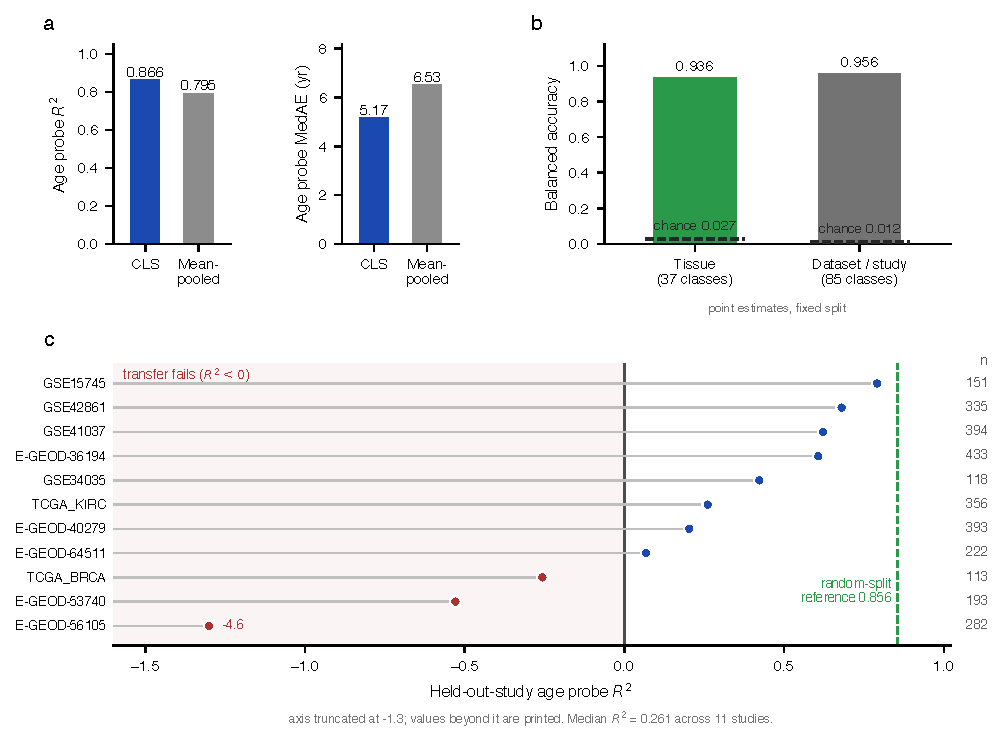
\includegraphics[width=\linewidth]{fig4_representation_cross_study_transfer.pdf}
 \caption{\textbf{Biological structure, study structure, and the limits of cross-study
 transfer.} \textbf{a}, Frozen linear age-probe performance using the pretrained CLS
 representation or mean-pooled contextual CpG embeddings, fitted on 8,724 and evaluated on
 2,264 profiles of the original AltuMAge partition. \textbf{b}, Balanced accuracy of frozen CLS
 linear probes for tissue (37 classes, 2,197 profiles) and dataset identity (85 classes, 2,006
 profiles); dashed segments mark the corresponding chance levels. The two tasks differ in class
 number and evaluation size and are not directly comparable to one another. \textbf{c},
 Leave-one-dataset-out age-probe $R^2$ for the 11 studies meeting the prespecified size
 ($n\geq100$) and age-dispersion (SD $\geq10$ years) thresholds, ordered by $R^2$; each row is
 one held-out study, with its cohort size given alongside. The dashed vertical line is the
 in-distribution random-split reference ($R^2=0.856$) and the solid line marks $R^2=0$; studies
with negative $R^2$ are shown in the shaded region. The axis is truncated at $R^2=-1.3$ and the
more extreme value is printed at the boundary. All panels report fixed-split point estimates from a single
frozen encoder; these analyses diagnose the pretrained representation and do not constitute
 external validation of the fine-tuned model.}
 \label{fig:representation-generalization}
\end{figure}
